\documentclass[10pt,aspectratio=169]{beamer}
\usepackage[utf8]{inputenc}
\usepackage[T1]{fontenc}
\usepackage[utf8]{vietnam}
\usepackage{graphicx}
\usepackage{booktabs}
\usepackage{amsmath,amssymb}
\usepackage{tikz}
\usepackage{colortbl}
\usepackage{pifont}
\usetikzlibrary{shapes,arrows,positioning,fit,calc,shadows}

\usetheme{Madrid}
\usecolortheme{whale}
\setbeamertemplate{navigation symbols}{}
\setbeamertemplate{headline}{}
\setbeamertemplate{footline}[frame number]

\hbadness=10000
\hfuzz=200pt
\vbadness=10000
\vfuzz=300pt

% The built-in editor compiles the main source in an isolated directory and
% may not copy project images. Keep the real figures in normal/local builds,
% while allowing that isolated preview to compile with an explicit placeholder.
\newcommand{\projectimage}[2][]{%
  \IfFileExists{#2}{\includegraphics[#1]{#2}}{%
    \fbox{\parbox[c][0.42\textheight][c]{0.88\linewidth}{%
      \centering\small External figure unavailable in isolated preview:\\[0.2cm]
      \texttt{\detokenize{#2}}}}}%
}

\definecolor{edgeblue}{RGB}{0,102,204}
\definecolor{edgered}{RGB}{204,0,0}
\definecolor{edgegreen}{RGB}{0,153,76}
\definecolor{edgegray}{RGB}{128,128,128}

\title{\textbf{EdgeSlice}: DAG-Aware Tensor Slicing for\\Memory-Constrained Edge Inference via MLIR Transform Dialect}
\subtitle{Compiler-Guided Memory Optimization for Edge Inference}
\author{
    \textbf{Supervisor:} Assoc. Prof. Dr. Quan Thanh Tho \\[0.2cm]
    \textbf{Members:} Cao Que Phuong, Truong Le Dan Chi, Mai Nguyen Tien Dat, \\
    Nguyen Minh Thai, Nguyen Thanh Toan, Le Cong Vinh
}
\institute{HCMUT}
\date{}

\begin{document}

% ==================== TITLE SLIDE ====================
\begin{frame}
\titlepage
\end{frame}

% ==================== OUTLINE ====================
\begin{frame}{Outline}
\begin{columns}[T,totalwidth=0.88\textwidth]
\begin{column}{0.42\textwidth}
\begin{enumerate}
\item Problem Statement
\item Literature Review
\item EdgeSlice Architecture
\item DAG Representation
\item Liveness Analysis
\end{enumerate}
\end{column}
\begin{column}{0.42\textwidth}
\begin{enumerate}
\setcounter{enumi}{5}
\item Tiling Strategy
\item Transform Generation
\item Experimental Evaluation
\item Ablation / Discussion
\item Conclusion
\end{enumerate}
\end{column}
\end{columns}
\end{frame}

% ==================== PROBLEM ====================
\section{Problem Statement}
\begin{frame}{The Edge Inference Memory Crisis}
\begin{itemize}
\item Edge devices typically have \textbf{limited on-chip cache/SRAM} relative to modern intermediate activations
\item Large intermediate tensors create bandwidth and capacity pressure on slower memory levels
\item Excess memory traffic can increase latency and reduce inference efficiency
\end{itemize}
\begin{center}
\textbf{Goal}: Keep the active tensor working set closer to on-chip memory capacity through compiler-guided slicing.
\end{center}
\end{frame}

% ==================== LITERATURE REVIEW ====================
\section{Literature Review}
\begin{frame}{Literature Review}
\begin{columns}
\column{0.5\textwidth}
\textbf{Tensor and Memory Optimization}
\begin{itemize}
\small
\item \textcolor{edgegreen}{Tensor slicing / loop tiling}: improve locality
\item \textcolor{edgegreen}{Live-range analysis}: reason about tensor lifetimes
\item \textcolor{edgegreen}{Automatic optimization}: TVM and MLIR
\end{itemize}

\vspace{0.25cm}
\textbf{Compiler Infrastructure}
\begin{itemize}
\small
\item MLIR Linalg-on-Tensors representation
\item MLIR Transform Dialect for declarative rewrites
\end{itemize}

\column{0.5\textwidth}
\textbf{Related Slicing Approaches}
\begin{itemize}
\small
\item \textcolor{edgeblue}{SConv}: convolution-focused slicing
\item \textcolor{edgeblue}{SConvTransform}: operator-level MLIR transform
\item \textcolor{edgeblue}{TSO}: graph-level tensor optimization
\item \textcolor{edgeblue}{TVM}: schedule search and autotiling
\end{itemize}

\vspace{0.25cm}
\begin{beamercolorbox}[sep=0.35em,center,rounded=true,shadow=true]{block body}
\small
\textbf{Gap}: Existing methods do not combine whole-DAG tensor lifetime analysis, memory-triggered slicing, and flexible MLIR Transform Dialect rewriting.
\end{beamercolorbox}
\end{columns}
\end{frame}

% ==================== RESEARCH GAP ====================
\begin{frame}{Research Gap: Current Methods Limitations}
\centering
\textbf{\large Whole-DAG Tensor Lifetimes Are Missing from Operator-Level Slicing}

\vspace{0.4cm}
\resizebox{0.97\textwidth}{!}{%
\begin{tabular}{l c c c c c}
\toprule
\textbf{Feature} & \textbf{SConv} & \textbf{SConvTransform} & \textbf{TSO} & \textbf{TVM AutoTiling} & \textbf{\textcolor{edgeblue}{EdgeSlice}} \\
\midrule
\rowcolor{gray!10}
Optimization Scope & Conv/operator & Conv/operator & Global graph & Global graph & \textbf{Full operation DAG} \\
\midrule
Tensor Liveness & \textcolor{edgered}{$\times$} & \textcolor{edgered}{$\times$} & \textcolor{edgered}{$\times$} & \textcolor{edgered}{$\times$} & \textcolor{edgegreen}{$\checkmark$} \\
\midrule
\rowcolor{gray!10}
Slicing Trigger & Operator rule & Operator rule & Global optimizer & Schedule search & \textbf{Memory pressure} \\
\midrule
Rewrite Mechanism & Backend & MLIR Transform & XLA/LLVM & TVM schedule & \textbf{MLIR Transform} \\
\midrule
Hardware Model & Fixed targets & Arch.-dependent & Specific NPU & Tuned setup & \textbf{Configurable cache budget} \\
\bottomrule
\end{tabular}}

\vspace{0.4cm}
\begin{beamercolorbox}[sep=0.45em,center,rounded=true,shadow=true]{block body}
\small
\textbf{Key Insight:} Whole-DAG lifetimes identify which tensors contribute most to peak memory pressure before a legal slicing strategy is selected.
\end{beamercolorbox}
\end{frame}

% ==================== ARCHITECTURE ====================
\section{EdgeSlice Architecture}
\begin{frame}{EdgeSlice System Overview}
\centering
{\Large \textbf{EdgeSlice Compiler Pipeline}}

\vspace{0.15cm}
\small PyTorch model $\rightarrow$ torch-mlir / Linalg-on-Tensors $\rightarrow$ DAG analysis $\rightarrow$ Transform rewrite $\rightarrow$ optimized MLIR

\vspace{0.15cm}
\projectimage[width=0.95\textwidth,height=0.70\textheight,keepaspectratio]{img/pipeline.png}
\end{frame}

\begin{frame}{Key Idea}
\begin{columns}[T,totalwidth=0.9\textwidth]
\begin{column}{0.43\textwidth}
\begin{itemize}
\item \textbf{DAG-Aware Analysis}\\
Global liveness and peak live tensor memory estimation
\item \textbf{Dimension-Aware Heuristic}\\
Batch $\to$ Spatial $\to$ Channel priority
\end{itemize}
\end{column}
\begin{column}{0.43\textwidth}
\begin{itemize}
\item \textbf{Declarative Transforms}\\
Rewriting through MLIR Transform Dialect
\item \textbf{Pre-Bufferization}\\
Tensor-level transforms remain composable with downstream lowering
\end{itemize}
\end{column}
\end{columns}
\end{frame}

% ==================== DAG ====================
\section{DAG Representation}
\begin{frame}{Operation DAG: Capturing Tensor Dependencies}
\begin{columns}
\begin{column}{0.45\textwidth}
\textbf{Data Structures:}
\begin{itemize}
\small
\item \texttt{nodes}: Dict[int, OpNode]
\item \texttt{edges}: List[(producer, consumer)]
\end{itemize}

\vspace{0.25cm}
\textbf{OpNode contains:}
\begin{itemize}
\small
\item \texttt{op\_id}: unique identifier
\item \texttt{op\_type}: conv\_2d, matmul, etc.
\item \texttt{input\_tensors}: List[TensorInfo]
\item \texttt{output\_tensor}: TensorInfo
\item \texttt{consumers}: List[int]
\end{itemize}

\vspace{0.25cm}
\textbf{Why DAG?}
\begin{itemize}
\small
\item Directed producer--consumer data flow
\item Feed-forward operation graph is acyclic
\item One output may remain live across multiple consumers
\end{itemize}
\end{column}

\begin{column}{0.55\textwidth}
\centering
\textbf{Key Properties:}
\vspace{0.4cm}
\begin{itemize}
\item \textbf{Nodes}: operations (conv, matmul, etc.)
\item \textbf{Edges}: tensor dependencies
\item \textbf{Topology}: execution-compatible ordering
\item \textbf{Memory}: enables lifetime analysis
\end{itemize}

\vspace{0.4cm}
\begin{block}{Example}
\small
Op0 produces T0 $\to$ consumed by Op1 and Op2\\
T0 remains live until its last downstream consumer completes.
\end{block}
\end{column}
\end{columns}
\end{frame}

% ==================== PARSER 1 ====================
\begin{frame}{From PyTorch to DAG: Native MLIR Python Bindings}
\centering
\textbf{MLIR-Powered DAG Construction Pipeline}
\vspace{0.25cm}
\begin{columns}
\begin{column}{0.5\textwidth}
\textbf{Implementation Approach:}
\begin{itemize}
\small
\item \textcolor{edgegreen}{\textbf{Native MLIR bindings}}: direct IR traversal
\item \textcolor{edgegreen}{\textbf{LINALG\_ON\_TENSORS}}: structured lowering target
\item \textcolor{edgegreen}{\textbf{SSA tracking}}: producer--consumer relationships
\item \textcolor{edgegreen}{\textbf{Attribute extraction}}: direct property access
\end{itemize}

\vspace{0.15cm}
\textbf{No String/Regex Parsing:}
\begin{itemize}
\small
\item Avoids fragile text patterns
\item Type-aware operation access
\item Robust edge construction
\end{itemize}
\end{column}

\begin{column}{0.5\textwidth}
\textbf{Parser Benchmark:}
\begin{itemize}
\small
\item \textbf{76 operations} parsed
\item \textbf{82 edges} connected
\item \textbf{9 operations} with parameters extracted
\item \textbf{421 ms} average parsing time
\item \textbf{100\%} topological ordering accuracy
\end{itemize}

\vspace{0.15cm}
\textbf{Attribute Extraction:}
\begin{itemize}
\tiny
\item \texttt{linalg.conv\_2d}: strides and dilations
\item \texttt{linalg.pooling}: strides and dilations
\end{itemize}

\vspace{0.15cm}
\textcolor{edgegreen}{\textbf{$\checkmark$ Native MLIR-Based Implementation}}
\end{column}
\end{columns}

\vspace{0.25cm}
\begin{beamercolorbox}[sep=0.3em,center,rounded=true,shadow=true]{block body}
\small
\textbf{Key Point}: Native bindings replace fragile string parsing with direct SSA and attribute access.
\end{beamercolorbox}
\end{frame}

% ==================== PARSER 2 ====================
\begin{frame}{Native MLIR Parser: Technical Implementation}
\begin{columns}
\begin{column}{0.5\textwidth}
\textbf{Step 1: Lowering}
\begin{itemize}
\small
\item \texttt{torch-mlir.compile()} with \texttt{LINALG\_ON\_TENSORS}
\item Produces structured tensor operations for analysis
\end{itemize}

\vspace{0.15cm}
\textbf{Step 2: Programmatic Traversal}
\begin{itemize}
\small
\item Walk \texttt{op.regions $\to$ block.operations}
\item Access \texttt{op.operands} and \texttt{op.results}
\item Track SSA values without textual conversion
\end{itemize}

\vspace{0.15cm}
\textbf{Step 3: Attribute Extraction}
\begin{itemize}
\small
\item Read named attributes directly
\item Extract strides, dilations, and padding
\end{itemize}
\end{column}

\begin{column}{0.5\textwidth}
\textbf{Step 4: Topological Sorting}
\begin{itemize}
\small
\item Kahn's algorithm
\item Producer--consumer SSA relationships
\item \textbf{100\% edge validation accuracy}
\end{itemize}

\vspace{0.15cm}
\textbf{Performance Metrics:}
\begin{itemize}
\small
\item \textbf{421.2 ms} average
\item \textbf{378.3 ms} minimum
\item \textbf{66.5 ms} standard deviation
\end{itemize}

\vspace{0.15cm}
\begin{beamercolorbox}[sep=0.2em,center,rounded=true,shadow=true]{block body}
\tiny
\textbf{Operation Coverage:} 6 convolutions + 2 pooling ops parameterized; 18 generic + 14 empty + 6 pad operations detected; full DAG structure preserved.
\end{beamercolorbox}
\end{column}
\end{columns}

\vspace{0.25cm}
\begin{beamercolorbox}[sep=0.3em,center,rounded=true,shadow=true]{block body}
\small
\textbf{Result}: A robust MLIR-based parser for DAG construction and subsequent liveness analysis.
\end{beamercolorbox}
\end{frame}

% ==================== LIVENESS ====================
\section{Liveness Analysis}
\begin{frame}{Liveness Analysis: Computing Tensor Lifetimes}
\begin{columns}[T,totalwidth=0.9\textwidth]
\begin{column}{0.48\textwidth}
\textbf{Definition:}
\begin{itemize}
\small
\item A tensor is \textcolor{edgegreen}{\textbf{live}} from its producer operation to its \textit{last} consumer
\end{itemize}

\vspace{0.2cm}
\textbf{Algorithm:}
\begin{enumerate}
\small
\item Assign a unique tensor ID
\item Determine \texttt{[producer, last\_consumer]}
\item Construct \texttt{live\_at[op\_id]}
\end{enumerate}

\vspace{0.2cm}
\textbf{Output:}
\begin{itemize}
\small
\item Set of tensors simultaneously live at each operation
\item Basis for peak live tensor memory estimation
\end{itemize}
\end{column}

\begin{column}{0.38\textwidth}
\centering
\projectimage[width=\linewidth,height=0.75\textheight,keepaspectratio]{img/liveness.png}
\end{column}
\end{columns}
\end{frame}

\begin{frame}{Peak Memory Estimation: Finding Slicing Candidates}
\begin{columns}
\begin{column}{0.4\textwidth}
\textbf{At each operation:}
\[
\text{memory}[op]=\sum_{t\in\text{live\_at}[op]}\text{size}(t)
\]

\vspace{0.2cm}
\textbf{Candidate identification:}
\begin{itemize}
\small
\item Memory pressure exceeds a configured cache threshold
\item Operation has downstream consumers
\item Prioritize larger memory-pressure contributions
\end{itemize}

\vspace{0.2cm}
\textbf{Interpretation:}
\begin{itemize}
\small
\item \textcolor{edgegreen}{\textbf{Above threshold}}: consider slicing
\item \textcolor{edgeblue}{\textbf{Within threshold}}: no slicing trigger
\item Legality is checked separately
\end{itemize}
\end{column}

\begin{column}{0.6\textwidth}
\centering
\projectimage[width=1.25\linewidth,height=0.70\textheight,keepaspectratio]{img/liveness.png}
\small Above-threshold operations become candidates for legal dimension-aware slicing.
\end{column}
\end{columns}
\end{frame}

% ==================== TILING ====================
\section{Tiling Strategy}
\begin{frame}{Tile Size Calculation: Fitting into Cache Budget}
\begin{columns}
\begin{column}{0.53\textwidth}
\textbf{Simplified analytical model:}
\begin{enumerate}
\small
\item Bytes per H-unit:
\[
b_{H}=\prod_{d\neq H}\text{size}(d)\times4
\]
\item Approximate input + output working set: $2b_H$
\item Maximum tile extent: $T_{\max}=\lfloor B/(2b_H)\rfloor$
\item Select a legal extent not exceeding $T_{\max}$
\end{enumerate}

\textbf{Example:}
\begin{itemize}
\small
\item Tensor: \texttt{[1, 64, 512, 512]}, slice H
\item $1\times64\times512=32{,}768$ FP32 elements
\item $b_H=32{,}768\times4=131{,}072$ bytes $=128$ KB
\item Input + output: $128\times2=256$ KB per H-unit
\item For $B=512$ KB: $T_{\max}=512/256=2$
\item \textcolor{edgegreen}{\textbf{Selected tile size: $T=2$}}
\end{itemize}
\end{column}

\begin{column}{0.47\textwidth}
\centering
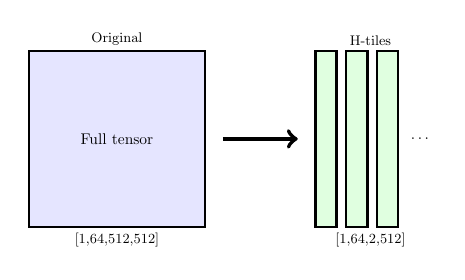
\begin{tikzpicture}[scale=0.56,transform shape]
\fill[blue!10] (0,0) rectangle (4,4);
\draw[thick] (0,0) rectangle (4,4);
\node at (2,2) {Full tensor};
\node[below] at (2,0) {\small [1,64,512,512]};
\node[above,font=\small] at (2,4) {Original};

\draw[->,thick,line width=1.5pt] (4.4,2)--(6.1,2);

\foreach \x in {6.5,7.2,7.9} {
  \fill[green!12] (\x,0) rectangle (\x+0.48,4);
  \draw[thick] (\x,0) rectangle (\x+0.48,4);
}
\node at (8.9,2) {$\cdots$};
\node[below,font=\small] at (7.75,0) {[1,64,2,512]};
\node[above,font=\small] at (7.75,4) {H-tiles};
\end{tikzpicture}

\vspace{0.35cm}
\begin{beamercolorbox}[sep=0.3em,center,rounded=true,shadow=true]{block body}
\footnotesize
\textbf{Note}: This is a simplified estimate; actual working sets may also include weights, halos, and temporary buffers.
\end{beamercolorbox}
\end{column}
\end{columns}
\end{frame}

\begin{frame}{Dimension Selection: Priority Heuristic}
\centering
{\Large \textbf{Slicing Priority:} \textcolor{edgeblue}{Batch} $\rightarrow$ \textcolor{edgegreen}{Spatial (H, W)} $\rightarrow$ \textcolor{edgered}{Channel}}

\vspace{0.2cm}
\projectimage[width=0.96\textwidth,height=0.62\textheight,keepaspectratio]{img/heuristic.png}

\vspace{0.1cm}
\begin{beamercolorbox}[sep=0.3em,center,rounded=true,shadow=true]{block body}
\small
\textbf{Batch}: samples are typically independent. \quad
\textbf{Spatial}: preserves locality but needs halo handling. \quad
\textbf{Channel}: may require accumulation or additional dependency handling.
\end{beamercolorbox}
\end{frame}

% ==================== HALO ====================
\begin{frame}{Halo-Aware Spatial Slicing}
\begin{columns}
\begin{column}{0.58\textwidth}
\centering
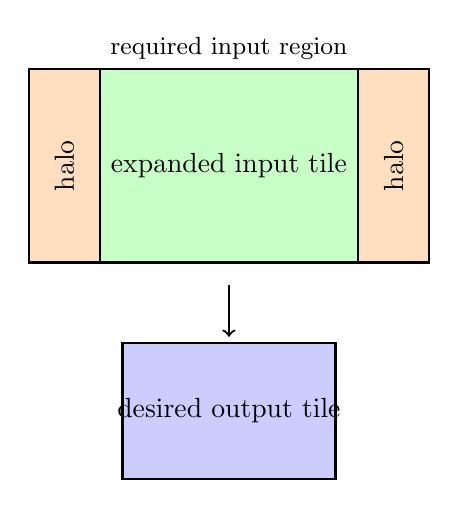
\begin{tikzpicture}[x=0.82cm,y=0.82cm]
\fill[orange!25] (0,0) rectangle (1.1,3.0);
\fill[green!22] (1.1,0) rectangle (5.1,3.0);
\fill[orange!25] (5.1,0) rectangle (6.2,3.0);
\draw[thick] (0,0) rectangle (6.2,3.0);
\draw[thick] (1.1,0)--(1.1,3.0);
\draw[thick] (5.1,0)--(5.1,3.0);
\node[rotate=90] at (0.55,1.5) {halo};
\node at (3.1,1.5) {expanded input tile};
\node[rotate=90] at (5.65,1.5) {halo};

\draw[->,thick] (3.1,-0.35)--(3.1,-1.15);
\fill[blue!20] (1.45,-3.35) rectangle (4.75,-1.25);
\draw[thick] (1.45,-3.35) rectangle (4.75,-1.25);
\node at (3.1,-2.3) {desired output tile};
\node[above,font=\small] at (3.1,3.0) {required input region};
\end{tikzpicture}
\end{column}

\begin{column}{0.42\textwidth}
\textbf{Why halos are needed:}
\begin{itemize}
\small
\item Kernel size, stride, dilation, and padding determine the required input region
\item The input region may extend beyond the nominal spatial tile
\item Adjacent tiles may overlap, introducing recomputation
\item Spatial slices are therefore not automatically independent
\end{itemize}

\vspace{0.25cm}
\begin{beamercolorbox}[sep=0.35em,center,rounded=true,shadow=true]{block body}
\small
\textbf{Goal}: Preserve convolution boundary correctness while controlling overlap overhead.
\end{beamercolorbox}
\end{column}
\end{columns}
\end{frame}

% ==================== TRANSFORMS ====================
\section{Transform Generation}
\begin{frame}[fragile]{Transform IR Generation}
\centering
\textbf{Tiled Rewrite Pattern:} \texttt{tile\_using\_forall} $\rightarrow$ \texttt{extract\_slice} $\rightarrow$ tiled op $\rightarrow$ \texttt{parallel\_insert\_slice}

\vspace{0.08cm}
\scriptsize
\begin{verbatim}
transform.structured.tile_using_forall %target
    tile_sizes [0, 0, 2, 0]

// Resulting payload pattern
scf.forall (%i) in (...) shared_outs(%out) {
  %slice = tensor.extract_slice %input[...]
  %tile = linalg.conv_2d
      ins(%slice, %filter) outs(%tile_out)
  scf.forall.in_parallel {
    tensor.parallel_insert_slice
      %tile into %out[...]
  }
}
\end{verbatim}

\vspace{-0.15cm}
\footnotesize The final tensor is assembled through disjoint output insertion semantics; \texttt{tensor.concat} is not inherently required.
\end{frame}

\begin{frame}[fragile]{Parallel Insert: Disjoint Result Assembly}
\textbf{Output discipline:}
\begin{itemize}
\small
\item Each tile targets a disjoint output region
\item Overlapping writes are not permitted
\item \texttt{tensor.parallel\_insert\_slice} expresses the insertion
\end{itemize}

\vspace{0.25cm}
\textbf{MLIR syntax:}
\small
\begin{verbatim}
scf.forall.in_parallel {
  tensor.parallel_insert_slice
    %tile into %result[%offset]
}
\end{verbatim}

\begin{beamercolorbox}[sep=0.3em,center,rounded=true,shadow=true]{block body}
\small
Disjoint output regions expose tile-level parallelism without conflicting writes.
\end{beamercolorbox}

\vspace{0.25cm}
\small Structured parallel semantics do not by themselves guarantee physical multithreading.
\end{frame}

% ==================== EARLY PROTOTYPE ====================
\begin{frame}{Early PyTorch Prototype / Preliminary Validation}
\begin{columns}
\begin{column}{0.5\textwidth}
\textbf{Prototype Components:}
\begin{itemize}
\small
\item \texttt{TensorSlicer}: runtime tensor tiling
\item \texttt{SlicedConv2d}, \texttt{SlicedLinear}: layer wrappers
\item \texttt{EdgeSlideTransform}: model-wide layer replacement
\item \texttt{MemoryProfiler}: preliminary per-layer profiling
\end{itemize}

\vspace{0.25cm}
\textbf{Purpose:}
\begin{itemize}
\small
\item Pure PyTorch feasibility prototype
\item Early validation of layer replacement and tiled execution
\item Supports Conv2d and Linear layers
\end{itemize}
\end{column}

\begin{column}{0.5\textwidth}
\textbf{Scope Boundary:}
\begin{itemize}
\small
\item Does not perform whole-DAG compiler liveness analysis
\item Does not represent the current primary contribution
\item Historical name: \textbf{EdgeSlide}
\end{itemize}

\vspace{0.4cm}
\begin{beamercolorbox}[sep=0.4em,center,rounded=true,shadow=true]{block body}
\small
\textbf{Current research focus}: compiler-level DAG analysis and MLIR Transform Dialect rewriting.
\end{beamercolorbox}
\end{column}
\end{columns}
\end{frame}

\begin{frame}{Runtime Overhead Analysis}
\begin{columns}
\begin{column}{0.5\textwidth}
\textbf{Potential Overheads:}
\begin{itemize}
\small
\item \textcolor{edgered}{Slice materialization}: depends on bufferization and lowering
\item \textcolor{edgered}{Loop overhead}: tiled iteration adds control flow
\item \textcolor{edgered}{Halo overlap}: may introduce recomputation
\item \textcolor{edgered}{Result assembly}: adds indexing and insertion work
\end{itemize}

\vspace{0.25cm}
\textbf{Mitigations / Benefits:}
\begin{itemize}
\small
\item Slice operations may lower to efficient views/subviews
\item \texttt{scf.forall} exposes structured tile-level parallelism
\item Smaller tiles aim to improve locality and reduce slower-memory pressure
\end{itemize}
\end{column}

\begin{column}{0.5\textwidth}
\textbf{Evaluation Interpretation:}
\begin{itemize}
\small
\item Cache residency is target- and lowering-dependent
\item Runtime RSS is not equivalent to L1 occupancy
\item Speedup is not guaranteed for every operator or platform
\end{itemize}

\vspace{0.35cm}
\begin{beamercolorbox}[sep=0.35em,center,rounded=true,shadow=true]{block body}
\small
\textbf{Trade-off}: Slice only when the expected reduction in active working set justifies tiling, halo, and loop overhead.
\end{beamercolorbox}
\end{column}
\end{columns}
\end{frame}

% ==================== EVALUATION ====================
\section{Experimental Evaluation}
% =====================================================================
%  MEASURED RESULTS
%
%  Replaces the former "Planned / Ongoing Evaluation" frame, whose three
%  items -- D1 cache behaviour, numerical correctness, IR-level memory --
%  are now measured.
%
%  Every figure below is measured on this repository at MLIR 19.1.1
%  against baseline commit 0b9e46b. Raw data:
%    benchmarks/results/evaluation_physical.json
%    benchmarks/results/deallocation_runtime_224.json
%    benchmarks/results/phase0_alloc_attribution_*_224.json
%    benchmarks/results/track_a_host_2026-09-30.json
%    benchmarks/results/track_a_sconv_2026-09-30.json
%    benchmarks/results/track_b_sram_2026-09-30.json
% =====================================================================

\begin{frame}{Post-Audit Implementation: What Is New}
\begin{columns}[T,totalwidth=0.99\textwidth]
\begin{column}{0.48\textwidth}
\textbf{Schedule generation}
\begin{itemize}
\small
\item Enumerate capacity-legal 1D/2D tile schedules
\item Rank by locality, traffic, vector utilisation, tile count, and budget utilisation
\item Preserve the historical first-feasible cascade as an ablation
\end{itemize}

\vspace{0.15cm}
\textbf{Target autotuning interface}
\begin{itemize}
\small
\item Measure an analytical shortlist on the target
\item Warm-up + repeated trials + median selection
\item Persistent cache keyed by target \emph{and workload}
\end{itemize}
\end{column}

\begin{column}{0.48\textwidth}
\textbf{Explicit SRAM placement}
\begin{itemize}
\small
\item Bufferize, then emit \texttt{transform.structured.promote}
\item Materialise \texttt{memref.alloc} in memory space 1
\item Materialise copy-in/copy-out operations
\item Compute the SRAM allocation high-water mark
\item Reject an artifact that exceeds usable SRAM
\end{itemize}

\vspace{0.15cm}
\begin{beamercolorbox}[sep=0.35em,center,rounded=true,shadow=true]{block body}
\small
The compiler no longer treats an annotation or a \texttt{memref.subview}
as evidence of physical SRAM placement.
\end{beamercolorbox}
\end{column}
\end{columns}
\end{frame}

\begin{frame}{New Evaluation Split: Track A and Track B}
\begin{columns}[T,totalwidth=0.99\textwidth]
\begin{column}{0.49\textwidth}
\textbf{Track A: executable CPU path}
\begin{itemize}
\small
\item Native AArch64 VM; Pi-4-like 32 KiB planning budget
\item Baseline and EdgeSlide lowered through the same MLIR/LLVM path
\item Five timed trials; eight kernel iterations per trial
\item Output checksums must match
\end{itemize}

\vspace{0.15cm}
\centering
\resizebox{\textwidth}{!}{%
\begin{tabular}{l r r r}
\toprule
\textbf{Kernel} & \textbf{Base} & \textbf{EdgeSlide} & \textbf{$\Delta$} \\
\midrule
TinyConv & 16.459 ms & 16.466 ms & $-0.05\%$ \\
SimpleCNN & 1834.11 ms & 1875.54 ms & $-2.26\%$ \\
Depthwise-64 & 5.986 ms & 6.007 ms & $-0.34\%$ \\
\bottomrule
\end{tabular}}
\end{column}

\begin{column}{0.47\textwidth}
\textbf{Track B: explicit SRAM artifact}
\begin{itemize}
\small
\item 32 KiB SRAM; 16 KiB usable slot when double-buffer capacity is reserved
\item TinyConv: 114 candidates, 1 SRAM allocation, 3 copies, 2,048 B peak
\item ConvStack: 384 candidates, 7 SRAM allocations, 14 copies, 15,360 B peak
\item Both pass capacity verification
\end{itemize}

\vspace{0.15cm}
\begin{beamercolorbox}[sep=0.35em,center,rounded=true,shadow=true]{block body}
\small
\textbf{Honest boundary:} no Track-B latency yet. The current host has no
GAP9/DIANA backend or DMA runtime. Ping-pong capacity is reserved, but the
DMA pipeline is not materialised.
\end{beamercolorbox}
\end{column}
\end{columns}

\vspace{0.2cm}
\begin{beamercolorbox}[sep=0.3em,center,rounded=true,shadow=true]{block body}
\small
Track-A mean speedup is \textbf{$-0.88\%$}: legality and placement are now
stronger, but the current schedule does not yet overcome loop/copy overhead.
\end{beamercolorbox}
\end{frame}

\begin{frame}{Measurement Scope: Three Numbers, Not One}
\begin{columns}[T,totalwidth=0.99\textwidth]
\begin{column}{0.52\textwidth}
Each evaluated cell now reports three quantities with \textbf{stated scope}:
\begin{enumerate}
\small
\item \textcolor{edgegray}{\textbf{Frontend estimate}} --- the analytical model. A \emph{predictor}.
\item \textcolor{edgeblue}{\textbf{Bufferized peak}} --- real \texttt{memref.alloc} sizes with last-use lifetimes.
\item \textcolor{edgegreen}{\textbf{Measured RSS}} --- OS high-water mark of the compiled binary.
\end{enumerate}

\vspace{0.2cm}
A cell that cannot be measured is recorded as \textbf{unmeasured}, never
back-filled with the estimate.
\end{column}

\begin{column}{0.44\textwidth}
\textbf{The three are not one quantity measured three ways.}

\vspace{0.15cm}
\small
Bufferized peak counts heap allocations. RSS counts every resident page ---
weight globals included, and those live in read-only data where no tiling
scheme can move them.

\vspace{0.15cm}
\centering
\resizebox{\textwidth}{!}{%
\begin{tabular}{l r r}
\toprule
\textbf{Model} & \textbf{Weights} & \textbf{RSS dilution} \\
\midrule
\rowcolor{gray!10}
resnet18 & 46.8 MB & $23.7\times$ \\
resnet50 & 102.4 MB & $13.5\times$ \\
\rowcolor{gray!10}
mobilenet\_v2 & 14.2 MB & $3.8\times$ \\
efficientnet\_b0 & 21.3 MB & $5.2\times$ \\
\rowcolor{gray!10}
unet & 31.1 MB & $6.9\times$ \\
\bottomrule
\end{tabular}}
\end{column}
\end{columns}

\vspace{0.3cm}
\begin{beamercolorbox}[sep=0.35em,center,rounded=true,shadow=true]{block body}
\small
An $X\%$ change in the activation peak can move RSS by at most $X/\text{dilution}$.
Weight totals cross-check exactly against published parameter counts at 4 bytes each.
\end{beamercolorbox}
\end{frame}

\begin{frame}{Legacy DPS Path: Peak Memory Reduction}
\centering
\resizebox{0.93\textwidth}{!}{%
\begin{tabular}{l c c c c}
\toprule
\textbf{Model} & \textbf{Res} & \textbf{Bufferized peak red.} & \textbf{RSS red.} & \textbf{RSS untiled / tiled / fused} \\
\midrule
\rowcolor{gray!10}
resnet50 & 64 & \textbf{0.00\%} & $-0.01\%$ & 106.8 / 106.8 / 106.8 MB \\
resnet50 & 96 & \textbf{0.00\%} & $-0.25\%$ & 107.3 / 107.3 / 107.5 MB \\
\rowcolor{gray!10}
resnet18 & 64 & \textbf{0.00\%} & $-0.26\%$ & 47.8 / 47.9 / 47.9 MB \\
resnet18 & 96 & \textbf{0.00\%} & $-0.52\%$ & 48.2 / 48.3 / 48.4 MB \\
\rowcolor{gray!10}
mobilenet\_v2 & 64 & \textbf{0.00\%} & $+0.60\%$ & 20.1 / 20.1 / 20.0 MB \\
mobilenet\_v2 & 96 & \textbf{0.00\%} & $+0.43\%$ & 21.1 / 21.0 / 21.0 MB \\
\rowcolor{gray!10}
efficientnet\_b0 & 64 & \textbf{0.00\%} & $-0.10\%$ & 27.1 / 27.1 / 27.1 MB \\
efficientnet\_b0 & 96 & \textbf{0.00\%} & $-0.35\%$ & 28.1 / 28.0 / 28.2 MB \\
\rowcolor{gray!10}
unet & 64 & \textbf{0.00\%} & $+0.68\%$ & 34.6 / 34.4 / 34.4 MB \\
unet & 96 & \textbf{0.00\%} & $+4.98\%$ & 40.9 / 39.1 / 38.9 MB \\
\bottomrule
\end{tabular}}

\vspace{0.3cm}
\begin{beamercolorbox}[sep=0.4em,center,rounded=true,shadow=true]{block body}
\small
\textcolor{edgered}{\textbf{Bufferized peak reduction is 0.00\% in all ten cells.}}
Five models, two resolutions, no cell refused. An allocation-attribution sweep
behind it --- 3 arms $\times$ 7 bufferization variants $\times$ 5 models,
\textbf{104 of 105 cells} --- reaches the same result independently.
\end{beamercolorbox}
\end{frame}

\begin{frame}{Why the Legacy DPS Path Cannot Reduce the Peak}
\begin{columns}[T,totalwidth=0.99\textwidth]
\begin{column}{0.5\textwidth}
\textbf{The mechanism, read off the IR:}
\begin{itemize}
\small
\item \texttt{tensor.parallel\_insert\_slice} writes into a \textbf{full-size destination}
\item So the destination must be materialised at full size
\item The tile exists only as a \texttt{memref.subview} --- a \emph{view}, which allocates nothing
\end{itemize}

\vspace{0.2cm}
\textbf{Confirmed on ResNet-50:}
\begin{itemize}
\small
\item Tiling adds \textbf{33 allocations}, removes 0 ($+35.7$ MB)
\item \textcolor{edgered}{\textbf{Not one}} of the 33 is under the tile budget
\item Allocations smaller than the budget: \textbf{25 in both arms}
\item 78 of 139 allocations exist only to receive a \texttt{memref.copy}
\end{itemize}
\end{column}

\begin{column}{0.46\textwidth}
\centering
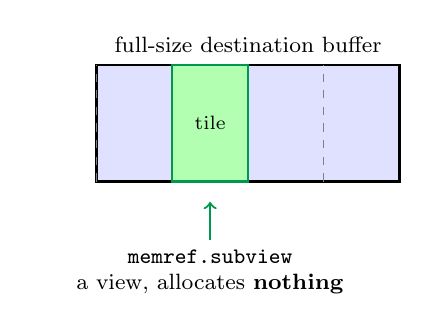
\begin{tikzpicture}[x=0.74cm,y=0.74cm,font=\small]
\fill[blue!12] (0,0) rectangle (5.2,2.0);
\draw[thick] (0,0) rectangle (5.2,2.0);
\node at (2.6,2.35) {\footnotesize full-size destination buffer};
\foreach \x in {0,1.3,2.6,3.9} {\draw[dashed,gray] (\x,0)--(\x,2.0);}
\fill[green!30] (1.3,0) rectangle (2.6,2.0);
\draw[thick,edgegreen] (1.3,0) rectangle (2.6,2.0);
\node[font=\scriptsize] at (1.95,1.0) {tile};
\draw[<-,thick,edgegreen] (1.95,-0.35)--(1.95,-1.0);
\node[below,font=\footnotesize,text width=4.4cm,align=center] at (1.95,-1.0)
  {\texttt{memref.subview}\\a view, allocates \textbf{nothing}};
\end{tikzpicture}

\vspace{1.05cm}
\begin{beamercolorbox}[sep=0.3em,center,rounded=true,shadow=true]{block body}
\footnotesize
Tiling can only \emph{add} buffers under DPS. It never shrinks one.
\end{beamercolorbox}
\end{column}
\end{columns}

\vspace{0.1cm}
\begin{beamercolorbox}[sep=0.25em,center,rounded=true,shadow=true]{block body}
\footnotesize
The 0.00\% is \textbf{structural for the legacy DPS path}. The new Track-B
path is separate: it promotes tiled operands into explicit scratchpad buffers
and verifies their allocation high-water mark.
\end{beamercolorbox}
\end{frame}

\begin{frame}{The Deallocation Gap: Where the Memory Actually Is}
\begin{columns}[T,totalwidth=0.99\textwidth]
\begin{column}{0.46\textwidth}
\textbf{Root cause:} \texttt{--buffer-deallocation} is a \texttt{func}-level pass.
The transform interpreter leaves the payload as
\texttt{module \{ module \{ func \} \}}, and a \texttt{func}-level pass
\textbf{silently skips} a function nested that deep --- exit 0, no diagnostic,
zero deallocations inserted.

\vspace{0.2cm}
The reported ``peak'' then degenerates to the \emph{sum of every allocation}.

\vspace{0.2cm}
\textbf{Minimal reproducer:} one \texttt{Conv2d}, 3 allocations.\\
wrapped $\rightarrow$ \textbf{0} deallocations.\\
unwrapped $\rightarrow$ \textbf{2}.
\end{column}

\begin{column}{0.5\textwidth}
\centering
\resizebox{\textwidth}{!}{%
\begin{tabular}{l r r r}
\toprule
\textbf{Model / arm} & \textbf{Heap before} & \textbf{after} & \textbf{$\times$} \\
\midrule
\rowcolor{gray!10}
resnet18 untiled & 31.3 MiB & 7.3 & 4.29 \\
resnet18 tiled & 36.2 MiB & 6.8 & 5.32 \\
\rowcolor{gray!10}
resnet50 untiled & 97.7 MiB & 17.4 & 5.61 \\
resnet50 tiled & 131.8 MiB & 17.4 & \textbf{7.57} \\
\rowcolor{gray!10}
mobilenet\_v2 untiled & 76.4 MiB & 9.9 & \textbf{7.72} \\
mobilenet\_v2 tiled & 99.2 MiB & 14.4 & 6.89 \\
\rowcolor{gray!10}
efficientnet\_b0 tiled & 101.9 MiB & 14.4 & 7.08 \\
unet untiled & 174.8 MiB & 39.1 & 4.47 \\
\rowcolor{gray!10}
unet tiled & 221.5 MiB & 39.1 & 5.66 \\
\bottomrule
\end{tabular}}

\vspace{0.15cm}
\footnotesize 9 of 14 arms shown; full range across all 14:\\
peak heap $4.12\times$--$7.72\times$, peak RSS $1.50\times$--$4.78\times$.
\end{column}
\end{columns}

\vspace{0.25cm}
\begin{beamercolorbox}[sep=0.4em,center,rounded=true,shadow=true]{block body}
\small
\textcolor{edgegreen}{\textbf{14 of 14 arms improve.}} Output checksums are
\textbf{bit-identical} before and after, and valgrind reports \textbf{0 errors}
on both binaries in every arm --- no invalid frees, no leaks.
\end{beamercolorbox}
\end{frame}

\begin{frame}{How the A/B Was Run}
\begin{columns}[T,totalwidth=0.99\textwidth]
\begin{column}{0.52\textwidth}
\textbf{Controlled comparison:} same payload, \textbf{one variable changed}
--- the pass list.

\vspace{0.2cm}
\begin{enumerate}
\small
\item Build arm A with the baseline pass list, arm B with the new one.
\item Run both: checksum, peak RSS (3 runs, minimum), peak heap via massif, valgrind error count.
\item \textcolor{edgered}{\textbf{Hash both binaries; refuse to compare unless they differ.}}
\item Delete the build tree before the next model.
\end{enumerate}

\vspace{0.2cm}
\small
Step 3 exists because a first attempt patched a constant the binary path does
not read. Both builds produced \emph{the same binary}, and every number from
that run --- a binary compared against itself --- was withdrawn.
\end{column}

\begin{column}{0.44\textwidth}
\textbf{Sample:} 5 models $\times$ 3 arms $=$ \textbf{14 measured arms}
(one refused for a dynamically-sized allocation).

\vspace{0.25cm}
\textbf{Not A/B tested:}
\begin{itemize}
\small
\item Wall-clock on a real Pi 4 --- no such hardware available for this work
\end{itemize}

\vspace{0.3cm}
\begin{beamercolorbox}[sep=0.4em,center,rounded=true,shadow=true]{block body}
\small
\textbf{Upstream baseline (G2):} SConvTransform builds against MLIR 19.1.1,
is numerically exact against the reference, and reaches \textbf{$17.4\times$}
the baseline kernel throughput. This is a convolution microbenchmark with a
local NEON runtime shim, not an end-to-end model claim.
\end{beamercolorbox}
\end{column}
\end{columns}
\end{frame}

\begin{frame}{Real Cache Geometry Changes the Framing}
\begin{columns}[T,totalwidth=0.99\textwidth]
\begin{column}{0.55\textwidth}
\centering
\resizebox{\textwidth}{!}{%
\begin{tabular}{l l r r r}
\toprule
\textbf{Model} & \textbf{Device} & \textbf{L1} & \textbf{L1-res.} & \textbf{2D-only} \\
\midrule
\rowcolor{gray!10}
resnet50 & pi4 & 32K & \textcolor{edgered}{\textbf{0}} & 1 \\
resnet50 & cortex\_a55 & 32K & \textcolor{edgered}{\textbf{0}} & \textbf{30} \\
\rowcolor{gray!10}
mobilenet\_v2 & pi4 & 32K & \textcolor{edgered}{\textbf{0}} & 0 \\
unet & pi4 & 32K & \textcolor{edgered}{\textbf{0}} & 3 \\
\rowcolor{gray!10}
unet & cortex\_a55 & 32K & \textcolor{edgered}{\textbf{0}} & \textbf{18} \\
efficientnet\_b0 & cortex\_a76 & 64K & \textcolor{edgered}{\textbf{0}} & 0 \\
\midrule
resnet50 & generic\_256k & 256K & 113 & 17 \\
\bottomrule
\end{tabular}}

\vspace{0.15cm}
\footnotesize Selected rows from a 4-device sweep over all five models.
\end{column}

\begin{column}{0.41\textwidth}
\textbf{At a real edge L1, nothing is L1-resident.}
\begin{itemize}
\small
\item The \texttt{L1-res} column is \textbf{0} for every model on every real device
\item Every accepted tile lives in L2 and streams through L1
\item The ``cache-resident tile'' framing survives only against a 256\,KB budget --- which is an \textbf{L2 size}
\end{itemize}

\vspace{0.2cm}
\textbf{The 2D cascade earns its place:}
\begin{itemize}
\small
\item On the 256\,KB-L2 Cortex-A55: 30 of 172 ResNet-50 anchors (17\%) and 18 of 68 U-Net anchors (26\%) have \textbf{no feasible 1D tile}
\end{itemize}
\end{column}
\end{columns}

\vspace{0.1cm}
\begin{beamercolorbox}[sep=0.25em,center,rounded=true,shadow=true]{block body}
\footnotesize
Any claim of the form ``tiles are made L1-resident'' has to be restated as
\textbf{L2-resident}, or the budget re-derived from a real 32\,KB L1.
\end{beamercolorbox}
\end{frame}

% ==================== DISCUSSION ====================
\section{Ablation / Discussion}
\begin{frame}{Ablation / Discussion: Selective Slicing}
\begin{columns}
\begin{column}{0.5\textwidth}
\textbf{Current Evidence}
\begin{itemize}
\small
\item \textcolor{edgegreen}{\textbf{EdgeSlice}} now searches capacity-legal 1D/2D schedules
\item Track B produces real non-default-memory-space allocations and copies
\item Track A is numerically correct but currently \textbf{0.88\% slower on average}
\item \textcolor{edgeblue}{\textbf{SConv}} remains substantially stronger at convolution-kernel optimisation
\end{itemize}
\end{column}

\begin{column}{0.5\textwidth}
\textbf{Required Next Ablations}
\begin{itemize}
\small
\item Search vs. historical first-feasible cascade
\item Analytical winner vs. target-measured winner
\item Liveness/fusion objective vs. per-layer tiling
\item Explicit SRAM promotion with and without DMA pipelining
\end{itemize}
\end{column}
\end{columns}

\vspace{0.35cm}
\begin{beamercolorbox}[sep=0.35em,center,rounded=true,shadow=true]{block body}
\small
\textbf{Interpretation}: the implementation evidence is now stronger than the
performance evidence. Correct placement is necessary, but is not itself a
speedup result.
\end{beamercolorbox}
\end{frame}

\begin{frame}{Reliability Method: Is the Safety Net a Net?}
\begin{columns}[T,totalwidth=0.99\textwidth]
\begin{column}{0.52\textwidth}
A guard nobody exercises is decoration. Each was \textbf{deliberately broken},
the suite re-run, and the mutation reverted.

\vspace{0.15cm}
\centering
\resizebox{\textwidth}{!}{%
\begin{tabular}{l c}
\toprule
\textbf{Mutated guard} & \textbf{Caught?} \\
\midrule
\rowcolor{gray!10}
unknown element type no longer raises & \textcolor{edgegreen}{$\checkmark$} \\
weight globals no longer counted & \textcolor{edgegreen}{$\checkmark$} \\
\rowcolor{gray!10}
module unwrap stops after one level & \textcolor{edgegreen}{$\checkmark$} \\
leaking payload no longer refused & \textcolor{edgegreen}{$\checkmark$} \\
\rowcolor{gray!10}
reporting path accepts inferred sizes & \textcolor{edgegreen}{$\checkmark$} \\
\textbf{payload no longer unwrapped} & \textcolor{edgered}{$\times$} \\
\bottomrule
\end{tabular}}

\vspace{0.05cm}
\footnotesize 6 of 10 mutations shown; 9 of 10 were caught.
\end{column}

\begin{column}{0.44\textwidth}
\textbf{The one that escaped} was the payload unwrap --- the guard whose
absence caused the original misdiagnosis. Deleting it left \textbf{all 475
fast tests passing}. It now has a test, and re-running the same mutation
against that test fails, so it is \emph{known} to catch what it was written
for.

\vspace{0.25cm}
\textbf{Claims withdrawn on re-measurement:}
\begin{itemize}
\small
\item ``tiling without fusion is worse in 8 of 8'' --- that spread was deallocation placement
\item ``the estimate ranks configurations correctly'' --- $r=+0.41$ at $p=0.15$ over 30 arms, not distinguishable from zero
\end{itemize}
\end{column}
\end{columns}

\vspace{0.1cm}
\begin{beamercolorbox}[sep=0.25em,center,rounded=true,shadow=true]{block body}
\footnotesize
A correlation was also once read off \textbf{15 arms left after 5 cells failed}.
Those cells were not missing at random --- they shared the property under
study. \textbf{A statistic over the cells that survived a failure is a
statistic about the failure.}
\end{beamercolorbox}
\end{frame}

% ==================== CONCLUSION ====================
\section{Conclusion}
\begin{frame}{Conclusion, Limitations \& Future Work}
\begin{columns}[T]
\begin{column}{0.33\textwidth}
\textbf{Main Contribution}
\begin{itemize}
\small
\item DAG-level tensor lifetime analysis
\item Capacity-safe 1D/2D schedule search
\item Fusion-budget legality checks
\item Verified MLIR SRAM placement
\end{itemize}
\end{column}

\begin{column}{0.31\textwidth}
\textbf{Current Evidence}
\begin{itemize}
\small
\item 507 non-hardware tests pass
\item Track A checksum equivalence on all three kernels
\item Track B capacity verification on both workloads
\item No measured EdgeSlide speedup yet
\end{itemize}
\end{column}

\begin{column}{0.34\textwidth}
\textbf{Limitations / Future Work}
\begin{itemize}
\small
\item Static-shape and analytical traffic assumptions
\item Run the autotuner on a physical target
\item Target DMA lowering and ping-pong buffers
\item MLPerf Tiny comparison with DORY/MATCH
\end{itemize}
\end{column}
\end{columns}
\end{frame}

\begin{frame}{Revised Conclusion}
\begin{columns}[T]
\begin{column}{0.33\textwidth}
\textbf{\textcolor{edgered}{Not supported}}
\begin{itemize}
\small
\item Peak-memory reduction from the legacy DPS tiling path: \textbf{0.00\%}
\item EdgeSlide latency superiority over SConv or untiled MLIR
\item ``L1-resident tiles'' at a real 32\,KB L1
\item Target-autotuned or DMA-overlapped execution
\end{itemize}
\end{column}

\begin{column}{0.33\textwidth}
\textbf{\textcolor{edgegreen}{Supported and measured}}
\begin{itemize}
\small
\item Whole-DAG liveness and the tooling to measure it
\item Search enumerates 114--384 candidates in Track B
\item Explicit SRAM allocations/copies; 2,048 B and 15,360 B verified peaks
\item Track-A output equivalence; mean latency change $-0.88\%$
\item SConvTransform reproduced at $17.4\times$ baseline kernel throughput
\end{itemize}
\end{column}

\begin{column}{0.33\textwidth}
\textbf{Where this points}
\begin{itemize}
\small
\item Current contribution: \textbf{auditable, capacity-safe compilation}, not a SOTA latency claim
\item Potential novelty is the combination of liveness, fusion budgeting, search, and verified placement
\item Next decisive experiment: physical SRAM target with DMA and measured autotuning
\end{itemize}
\end{column}
\end{columns}

\vspace{0.3cm}
\begin{beamercolorbox}[sep=0.4em,center,rounded=true,shadow=true]{block body}
\small
The negative result is the sharper contribution: it identifies \emph{why}
operator-level tiling cannot reduce peak memory in a destination-passing IR,
and it names what can.
\end{beamercolorbox}
\end{frame}

% ==================== BACKUP ====================
\appendix
\section{Backup}

\begin{frame}{Backup: Implementation Validation}
\begin{columns}
\begin{column}{0.5\textwidth}
\textbf{Preliminary / Historical Validation}
\begin{itemize}
\small
\item Standalone PyTorch models
\item CNN model: 23.4M parameters, 89.4 MB
\item LargeCNN used as an architecture proxy
\item Inputs: (1,3,224,224) and (1,64,512,512)
\end{itemize}

\vspace{0.25cm}
\textbf{Memory Measurement Limitation}
\begin{itemize}
\small
\item CPU allocation tracking was incomplete
\item Tensor-size and activation profiling were used only for preliminary validation
\item Both synthetic architectures have since been removed; all reported workloads use published checkpoints
\end{itemize}
\end{column}
\begin{column}{0.5\textwidth}
\begin{beamercolorbox}[sep=0.3em,center,rounded=true,shadow=true]{block body}
\small
\textbf{Historical Status}
\begin{itemize}
\small
\item \textcolor{edgegreen}{$\checkmark$} Tensor slicing prototype
\item \textcolor{edgegreen}{$\checkmark$} Automatic layer replacement
\item \textcolor{edgegreen}{$\checkmark$} Inference timing
\item \textcolor{edgeblue}{$\sim$} Memory estimate
\item \textcolor{edgered}{$\times$} Full custom-operator integration
\end{itemize}
\end{beamercolorbox}
\end{column}
\end{columns}
\end{frame}

\begin{frame}{Backup: Baseline Measurement Approach}
\begin{columns}
\begin{column}{0.5\textwidth}
\textbf{Preliminary / Historical Estimate}
\begin{itemize}
\small
\item Earlier work used \texttt{model\_size $\times$ 3.5}
\item This heuristic mixed parameter and activation estimates
\item It is \textbf{not} the current primary peak-memory methodology
\end{itemize}

\vspace{0.25cm}
\textbf{Current Methodology}
\begin{itemize}
\small
\item IR-level peak live tensor memory from DAG liveness
\item Runtime Peak RSS reported separately
\item D1 cache behavior measured separately
\end{itemize}
\end{column}

\begin{column}{0.5\textwidth}
\centering
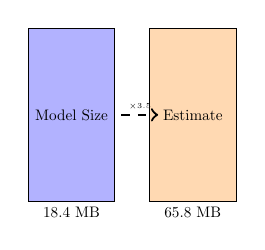
\begin{tikzpicture}[scale=0.55,transform shape]
\draw[fill=blue!30] (0,0) rectangle (2,4);
\node at (1,2) {Model Size};
\node[below] at (1,0) {18.4 MB};
\draw[fill=orange!30] (2.8,0) rectangle (4.8,4);
\node at (3.8,2) {Estimate};
\node[below] at (3.8,0) {65.8 MB};
\draw[->,thick,dashed] (2.15,2)--(3.0,2);
\node[above,font=\tiny] at (2.58,2) {$\times3.5$};
\end{tikzpicture}

\vspace{0.35cm}
\begin{beamercolorbox}[sep=0.25em,center,rounded=true,shadow=true]{block body}
\footnotesize Historical context only; no current memory-reduction claim is derived from this multiplier.
\end{beamercolorbox}
\end{column}
\end{columns}
\end{frame}

\begin{frame}{Backup: Theoretical vs. Prototype Results}
\begin{table}
\centering
\caption{Historical comparison; not the current primary evaluation}
\small
\begin{tabular}{l c c}
\toprule
\textbf{Metric} & \textbf{Earlier Estimate} & \textbf{PyTorch Prototype} \\
\midrule
Memory Method & Model-size multiplier & Hooks + tensor sizes \\
Inference Impact & Not established & Preliminary timing only \\
Layers Transformed & N/A & 8 auto-detected \\
Current Role & Historical context & Feasibility validation \\
\bottomrule
\end{tabular}
\end{table}

\begin{beamercolorbox}[sep=0.35em,center,rounded=true,shadow=true]{block body}
\small
Unsupported 88\% memory reduction and ``production-ready'' claims have been removed. Current evaluation separates DAG liveness, Peak RSS, cache behavior, and numerical correctness.
\end{beamercolorbox}
\end{frame}

\begin{frame}{Backup: Counter Resolvability}
\begin{columns}[T,totalwidth=0.99\textwidth]
\begin{column}{0.5\textwidth}
\textbf{Noise floor, measured}
\begin{itemize}
\small
\item Cachegrind is \emph{exact} for a fixed binary: three runs, identical counts
\item Across rebuilds it varies by \textbf{0.002--0.005\%}, because work-directory path length shifts memory layout
\item Reported cache effects clear that floor by \textbf{$13\times$--$5{,}775\times$}
\end{itemize}
\end{column}

\begin{column}{0.46\textwidth}
\textbf{Numerical equivalence}
\begin{itemize}
\small
\item Tolerance tightened from $10^{-3}$ to $10^{-4}$ after measuring all cells
\item Worst observed deviation: $1.53\times10^{-5}$ --- at least $7\times$ headroom
\item The achieved margin is logged on \emph{success}, not only on failure, so a regression that stays inside tolerance is still visible
\end{itemize}
\end{column}
\end{columns}

\vspace{0.25cm}
\begin{beamercolorbox}[sep=0.35em,center,rounded=true,shadow=true]{block body}
\small
A tolerance catches a regression that crosses it; a recorded margin makes one that stays inside it visible too.
\end{beamercolorbox}
\end{frame}

\begin{frame}{Backup: Interaction with Other Optimizations}
\begin{columns}
\begin{column}{0.5\textwidth}
\textbf{Quantization and Pruning}
\begin{itemize}
\small
\item EdgeSlice may be complementary to lower-precision tensors
\item Pruning may reduce weights or computation, depending on sparsity support
\item Combined effects must be measured by memory component; reduction factors are not multiplied automatically
\item \textit{Not yet integrated}
\end{itemize}
\end{column}

\begin{column}{0.5\textwidth}
\textbf{Operator Fusion}
\begin{itemize}
\small
\item Fusion and slicing can change intermediate lifetimes
\item The best ordering is target- and operator-dependent
\item Tile-level fusion and pipelining are future work
\item \textit{MLIR support exists; EdgeSlice integration is ongoing}
\end{itemize}
\end{column}
\end{columns}
\end{frame}

\end{document}
